\genHeader

Welcome to Part V of the eMoflon handbook, an introduction to bidirectional model-to-text transformations using Triple Graph Grammars (TGGs). If you're just
joining us and haven't completed any of the previous parts, we recommend working through at least Part I for the required setup and installation instructions
to ensure eMoflon is working correctly, and strongly encourage finishing Part IV to master the basics of TGGs. That part will be a key reference if you're ever
unsure how to use a TGG feature. Apart from TGG fundamentals however, we have assumed as little as possible from any of the previous parts and
include appropriate references where necessary.

Up until now in the handbook, we have created \texttt{LeitnersLearningBox}, a memorization tool that stores cards (with keywords on the front, and definitions
on the back) in different partitions, which then move through the box based on a set of rules simulating how our short and long-term memory works. This
metamodel was used in Part IV as a source language in a \emph{bidirectional}\define{Bidirectional Transformation}  TGG transformation, where each card was
translated into an entry (with a sole content attribute storing all its information) in a \texttt{Dictionary} metamodel. In this part, we shall implement a
second bidirectional transformation, this time a model-to-text transformation to establish a textual representation of the  \texttt{Dictionary} metamodel.
We'll use an \texttt{ANTLR}~\cite{ANTLR} parser and unparser, and TGGs to transform the parsed tree from ANTLR to an instance of the \texttt{Dictionary}
metamodel.

When establishing a model-driven solution, \emph{model transformations} usually play a central and important role. They could be used for specifying dynamic
semantics (as done for the rules of our learning box) or, more generally, for transforming a certain model to another model to achieve some goal (i.e.,
checking or guaranteeing consistency, adding or abstracting from platform details, \ldots).

There are many \emph{types} of model transformations and \cite{CH03,Mens_Gorp_2006} give a nice and detailed classification along a set of different dimensions.
In this part, we shall explore some of these dimensions and learn how \emph{model-to-text} transformations can be achieved with a nice mixture of \emph{string
grammars} and \emph{graph grammars}.

For the rest of this part, a model transformation is denoted as:
\begin{displaymath}
 	\Delta: m_{src} \rightarrow m_{trg}
\end{displaymath}
where the source model $m_{src}$ is to be transformed to the target model $m_{trg}$. Let's review the four primary ways in which $\Delta$ can be classified.

$\Delta$ is \emph{endogenous}\define{Endogenous}, if $m_{src}$ and $m_{trg}$ conform to the same metamodel. All story driven models (SDMs) built in Part III for
\texttt{LeitnersLearningBox} are examples of \emph{endogenous} transformations.

$\Delta$ is \emph{exogenous}\define{Exogenous}, if $m_{src}$ and $m_{trg}$ are instances of different metamodels. For example: A dictionary is used to learn new
words (similar to a learning box), but is more suitable for use as a reference (i.e., one already knows the words, but may occasionally need a specific
definition). In contrast, a learning box is geared towards the actual memorization process. Therefore, one could start with a learning box and, once all the
words have been memorized, transform it into a personalised dictionary for future reference. If too many words become forgotten, the dictionary should be
transformed back to a learning box. The learning box to dictionary transformation and vice-versa are therefore examples of \emph{exogenous} transformations, and
we implemented this in Part IV by using TGGs to transform our \texttt{LeitnersLearningBox} to a \texttt{Dictionary}.

$\Delta$ operates \emph{in-place}\define{In-place} if $m_{src}$ is \emph{destructively} transformed to $m_{trg}$. The SDMs for our learning box (e.g.,
\texttt{grow} or \texttt{check}) are examples of \emph{in-place} transformations as they perform destructive changes directly to a source model, transforming it
into the target model.

Finally, $\Delta$ is \emph{out-place}\define{Out-place} if $m_{src}$ is left intact and is unchanged by the transformation which creates $m_{trg}$. The
learning box to dictionary transformation with TGGs is an example of an \emph{out-place} transformation.

Although \emph{endogenous} + \emph{in-place} is the natural case for SDMs (as was the case for our learning box), \emph{exogenous} and/or \emph{out-place}
transformations can also be specified with SDMs. 
 
\newpage
 
To twist your brain a bit, here are a few interesting statements:
\begin{enumerate}

\item[$\blacktriangleright$] \emph{Out-place} transformations can be \emph{endogenous} or \emph{exogenous}.

\item[$\blacktriangleright$] \emph{In-place} transformations can usually only be \emph{endogenous}. \emph{Exo\-gen\-ous} transformations are consequently,
always \emph{out-place}.  Why?

\end{enumerate}  

It should be noted that $\Delta$ can be further classified as \emph{horizontal} if $m_{src}$ and $m_{trg}$ are on the same \emph{abstraction level}, or
\emph{vertical} if they are not. Unfortunately, this \emph{abstraction level} dimension is a bit `fuzzy,' but we will explore and work on these different levels
by establishing a textual concrete syntax for \texttt{Dictionary}. We shall learn how TGGs can be used in combination with parser generators
and template languages to implement model-to-text and text-to-model transformations that are typically \emph{vertical} (text is normally on a lower abstraction
level than a model). On the other hand, the overall learning box to dictionary transformation completed in the previous part (also with TGGs) is
\emph{horizontal} as the models represent the \emph{same} information differently, and can thus be considered to be on the same abstraction level.

% Fig.~\ref{fig:moca-overview} gives a ``big picture'' of what we plan to achieve in this part of the eMoflon handbook. All explanations are integrated right with
% the figure, so take your time to read it carefully and let it sink in. We'll be zooming in the bits and pieces of each step in the following sections to clear
% up any confusion.

% \begin{figure}[htp]
% \begin{center}
%  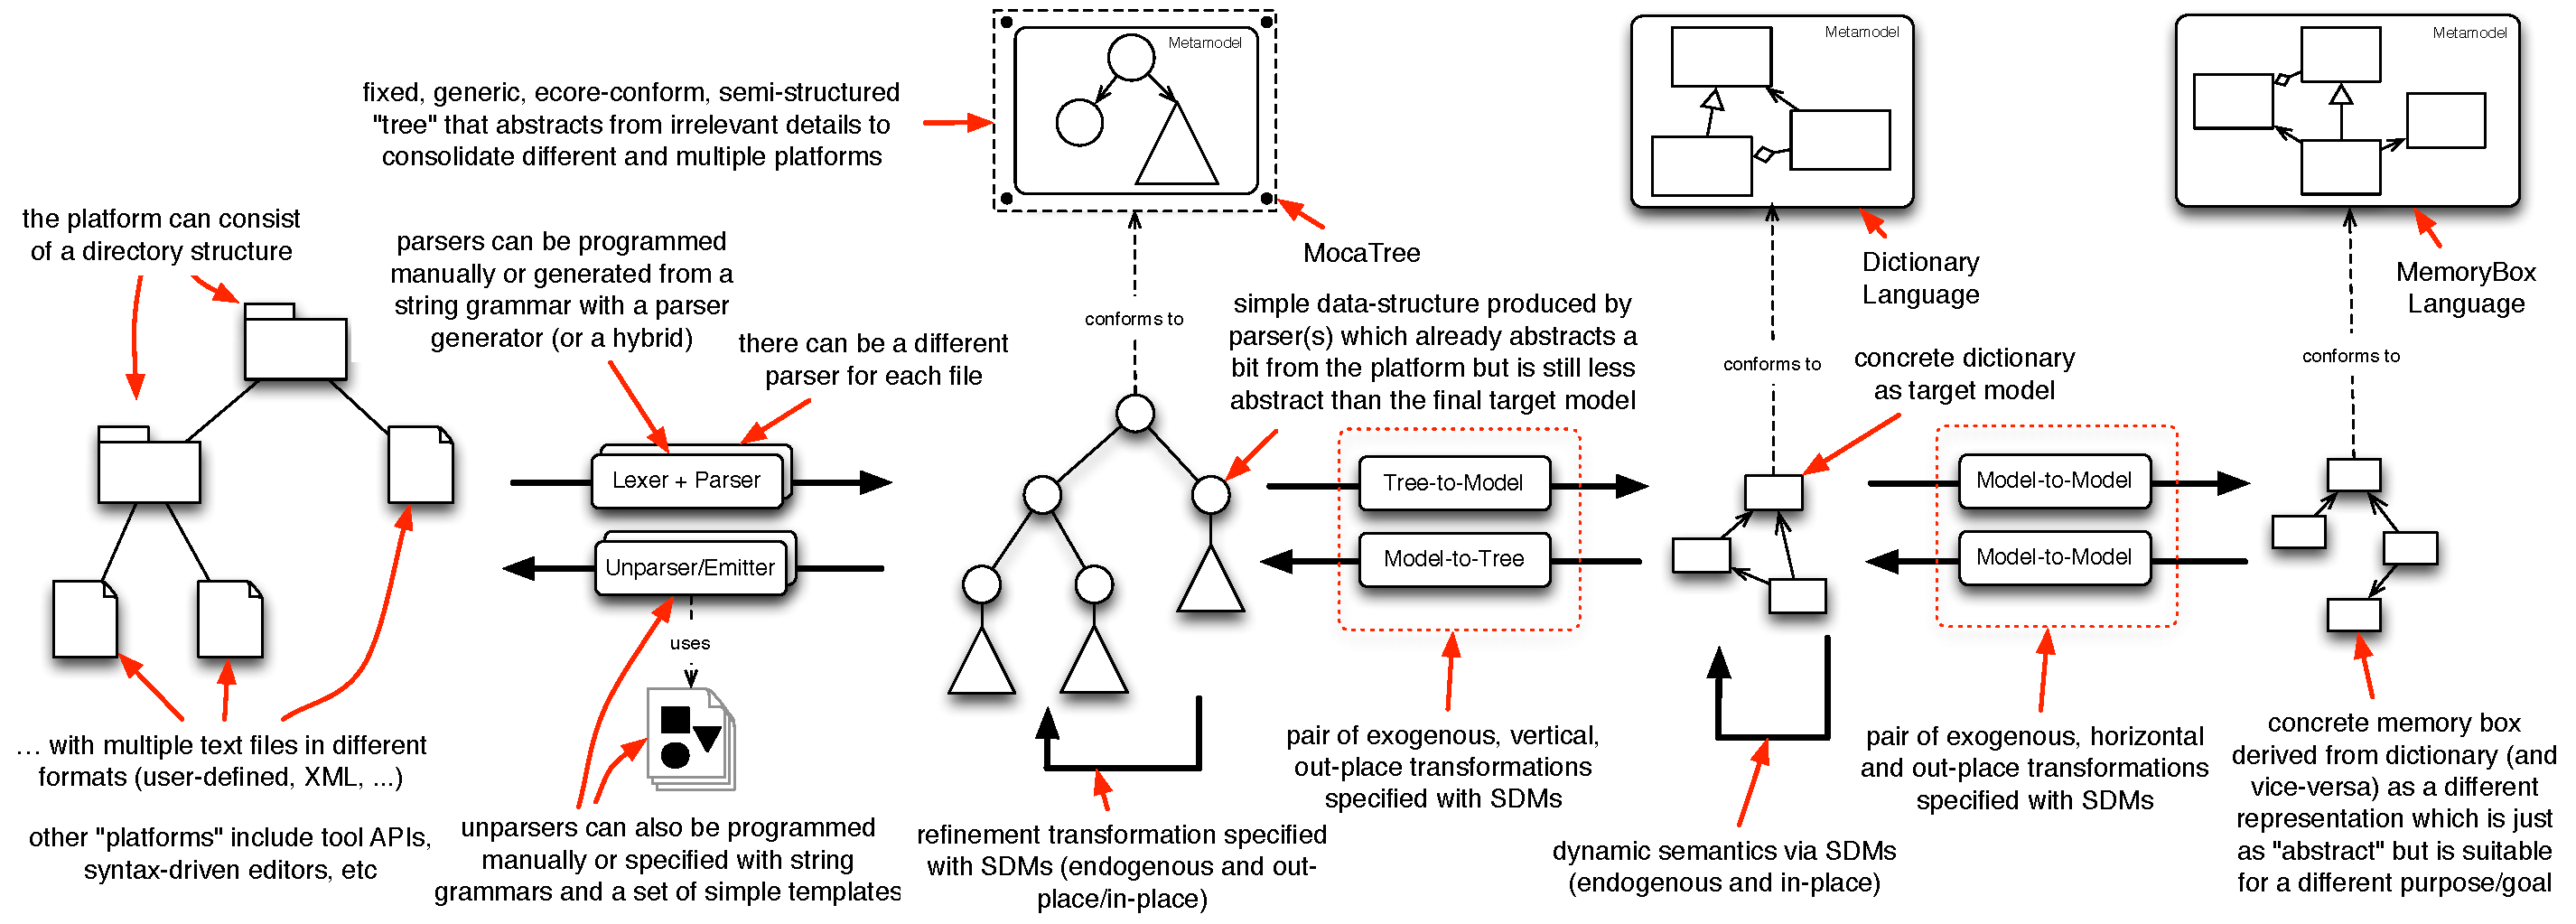
\includegraphics[angle=90, height=\textheight]{pics/moca/text-to-model}
%   \caption{Overview of model-to-text with the MOCA framework}
%   \label{fig:moca-overview}
% \end{center}
% \end{figure} 
